% ============================================================================
% Figuras Individuales de Filtros de PDI con Pie de Página y Descripción
% Generado automáticamente por Visualizer
% ============================================================================


\subsection*{Referencia Base}

\begin{figure}[htbp]
  \centering
  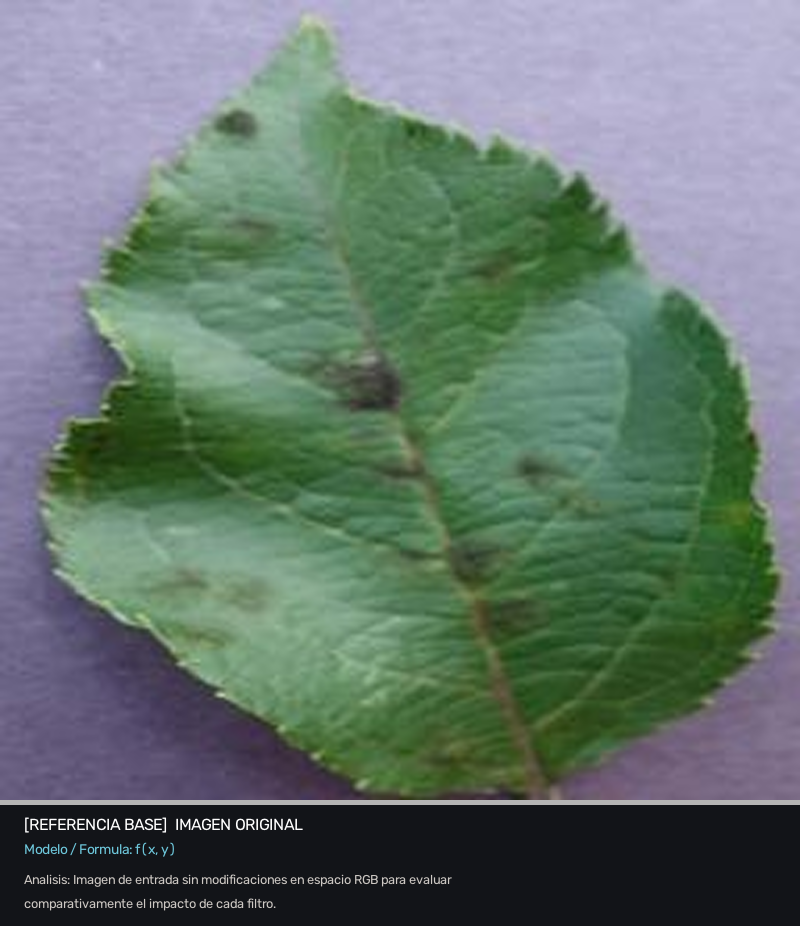
\includegraphics[width=0.78\linewidth]{resultados/individuales/muestra_01/01_original.png}
  \caption{\textbf{Imagen Original:} Imagen de entrada sin modificaciones en espacio RGB para evaluar comparativamente el impacto de cada filtro. \textit{Modelo:} \texttt{f(x, y)}.}
  \label{fig:01_original}
\end{figure}


\subsection*{Cat 1: Transformaciones de Intensidad}

\begin{figure}[htbp]
  \centering
  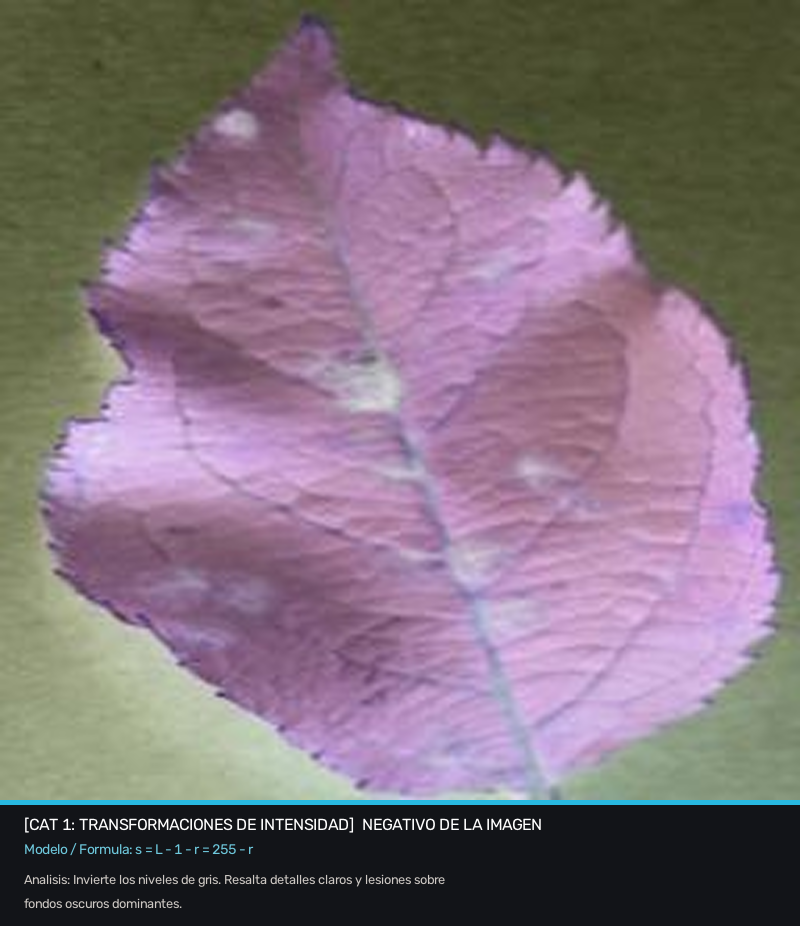
\includegraphics[width=0.78\linewidth]{resultados/individuales/muestra_01/02_negativo.png}
  \caption{\textbf{Negativo de la Imagen:} Invierte los niveles de gris. Resalta detalles claros y lesiones sobre fondos oscuros dominantes. \textit{Modelo:} \texttt{s = L - 1 - r = 255 - r}.}
  \label{fig:02_negativo}
\end{figure}

\begin{figure}[htbp]
  \centering
  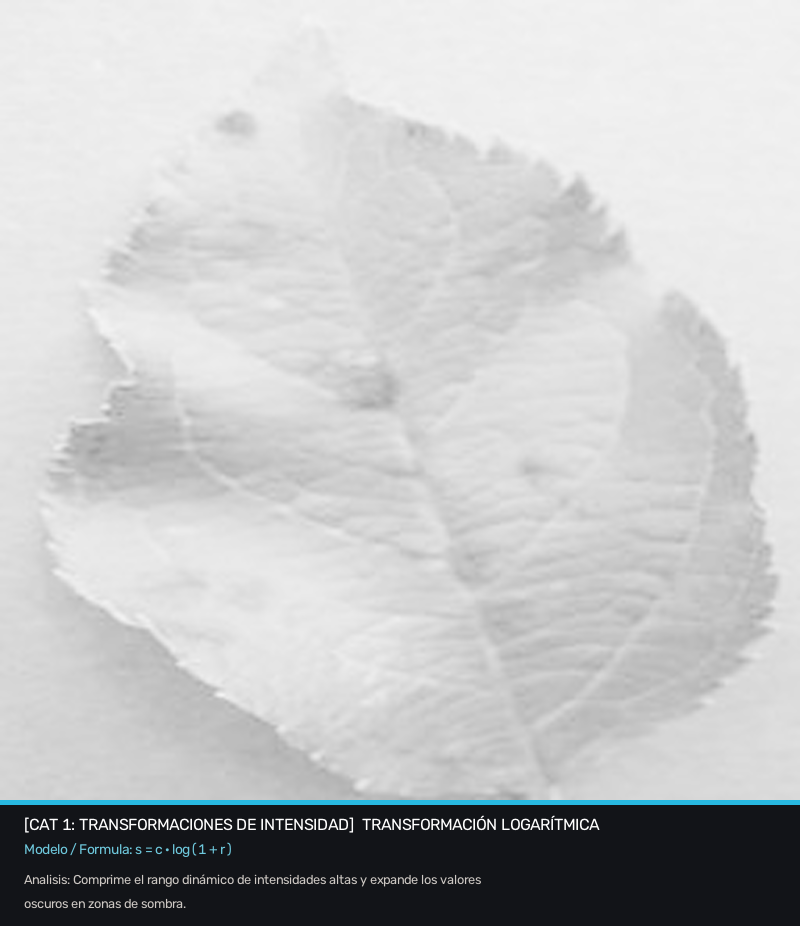
\includegraphics[width=0.78\linewidth]{resultados/individuales/muestra_01/03_logaritmico.png}
  \caption{\textbf{Transformación Logarítmica:} Comprime el rango dinámico de intensidades altas y expande los valores oscuros en zonas de sombra. \textit{Modelo:} \texttt{s = c · log(1 + r)}.}
  \label{fig:03_logaritmico}
\end{figure}

\begin{figure}[htbp]
  \centering
  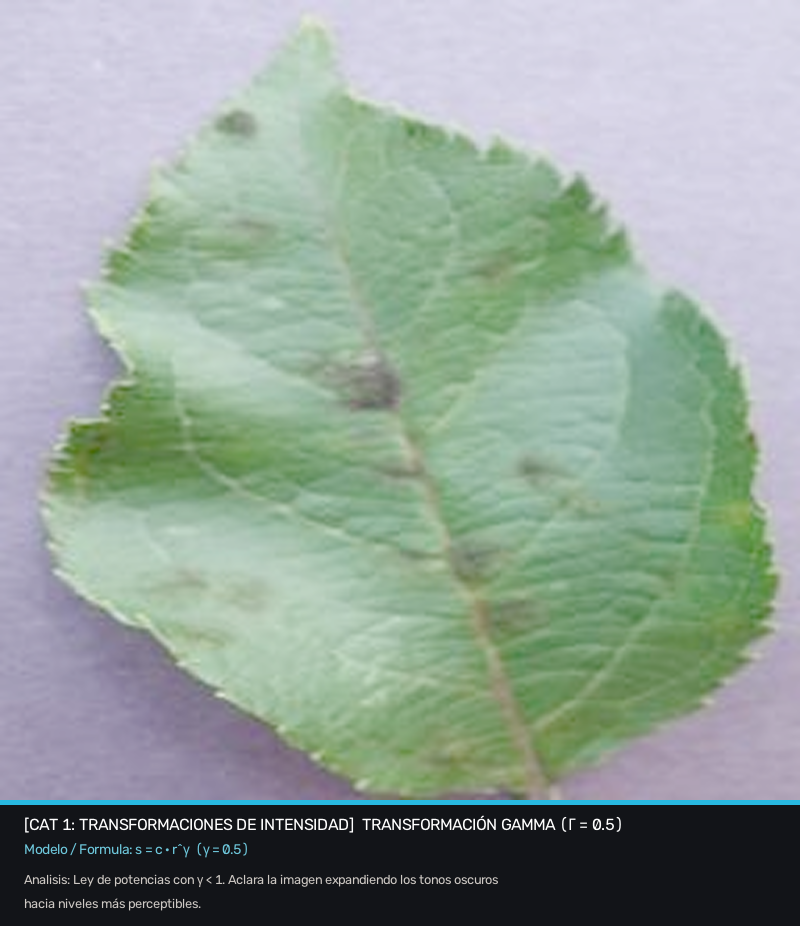
\includegraphics[width=0.78\linewidth]{resultados/individuales/muestra_01/04_gamma_aclara.png}
  \caption{\textbf{Transformación Gamma (γ = 0.5):} Ley de potencias con γ < 1. Aclara la imagen expandiendo los tonos oscuros hacia niveles más perceptibles. \textit{Modelo:} \texttt{s = c · r^γ  (γ = 0.5)}.}
  \label{fig:04_gamma_aclara}
\end{figure}

\begin{figure}[htbp]
  \centering
  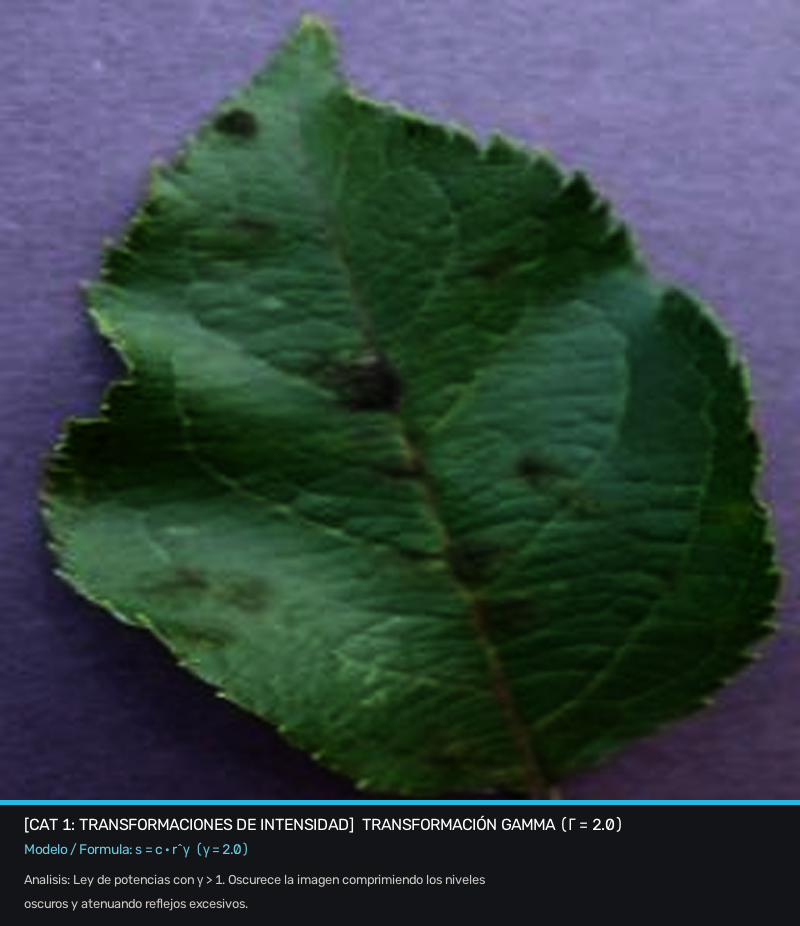
\includegraphics[width=0.78\linewidth]{resultados/individuales/muestra_01/05_gamma_oscurece.png}
  \caption{\textbf{Transformación Gamma (γ = 2.0):} Ley de potencias con γ > 1. Oscurece la imagen comprimiendo los niveles oscuros y atenuando reflejos excesivos. \textit{Modelo:} \texttt{s = c · r^γ  (γ = 2.0)}.}
  \label{fig:05_gamma_oscurece}
\end{figure}

\begin{figure}[htbp]
  \centering
  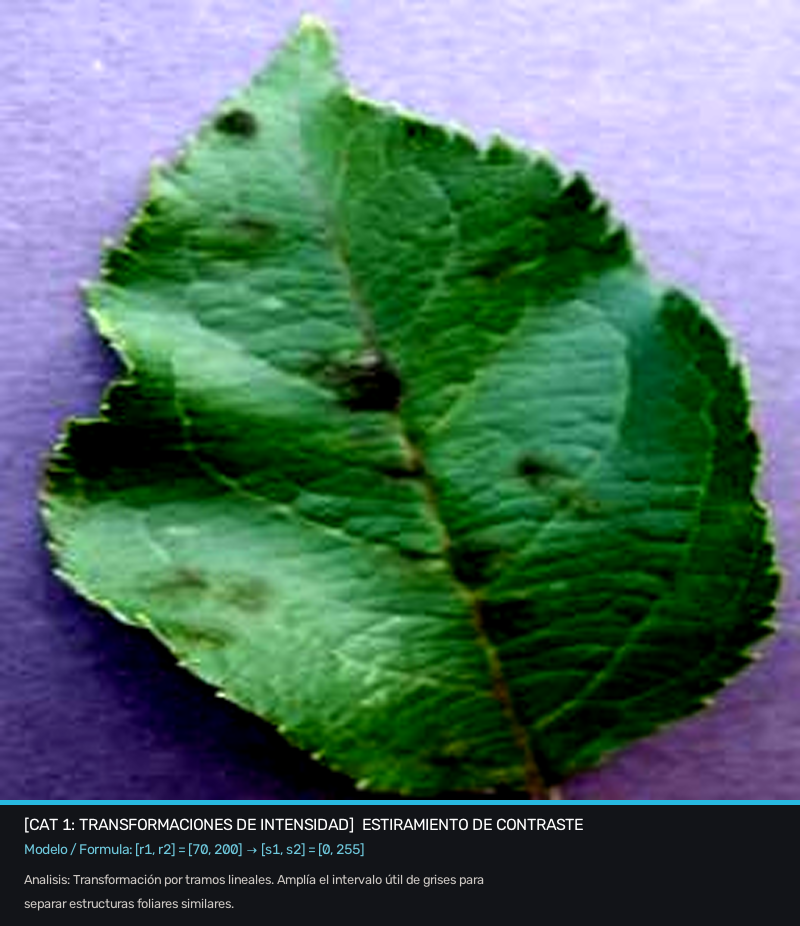
\includegraphics[width=0.78\linewidth]{resultados/individuales/muestra_01/06_estiramiento_contraste.png}
  \caption{\textbf{Estiramiento de Contraste:} Transformación por tramos lineales. Amplía el intervalo útil de grises para separar estructuras foliares similares. \textit{Modelo:} \texttt{[r1, r2] = [70, 200] → [s1, s2] = [0, 255]}.}
  \label{fig:06_estiramiento_contraste}
\end{figure}

\begin{figure}[htbp]
  \centering
  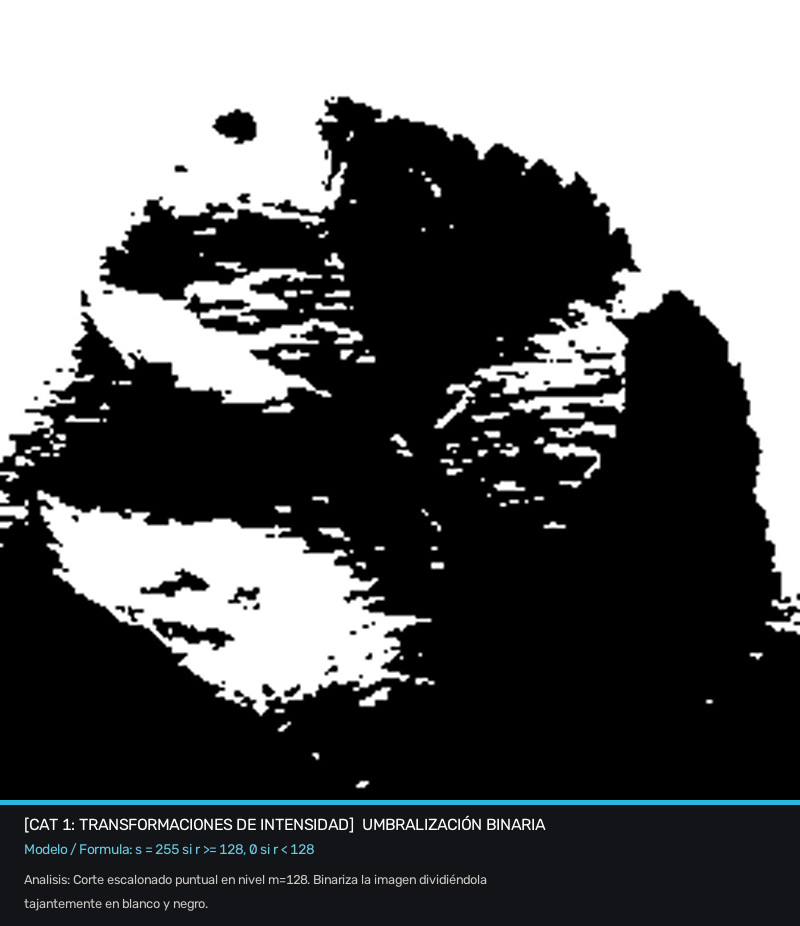
\includegraphics[width=0.78\linewidth]{resultados/individuales/muestra_01/07_umbral_binario.png}
  \caption{\textbf{Umbralización Binaria:} Corte escalonado puntual en nivel m=128. Binariza la imagen dividiéndola tajantemente en blanco y negro. \textit{Modelo:} \texttt{s = 255 si r >= 128, 0 si r < 128}.}
  \label{fig:07_umbral_binario}
\end{figure}

\begin{figure}[htbp]
  \centering
  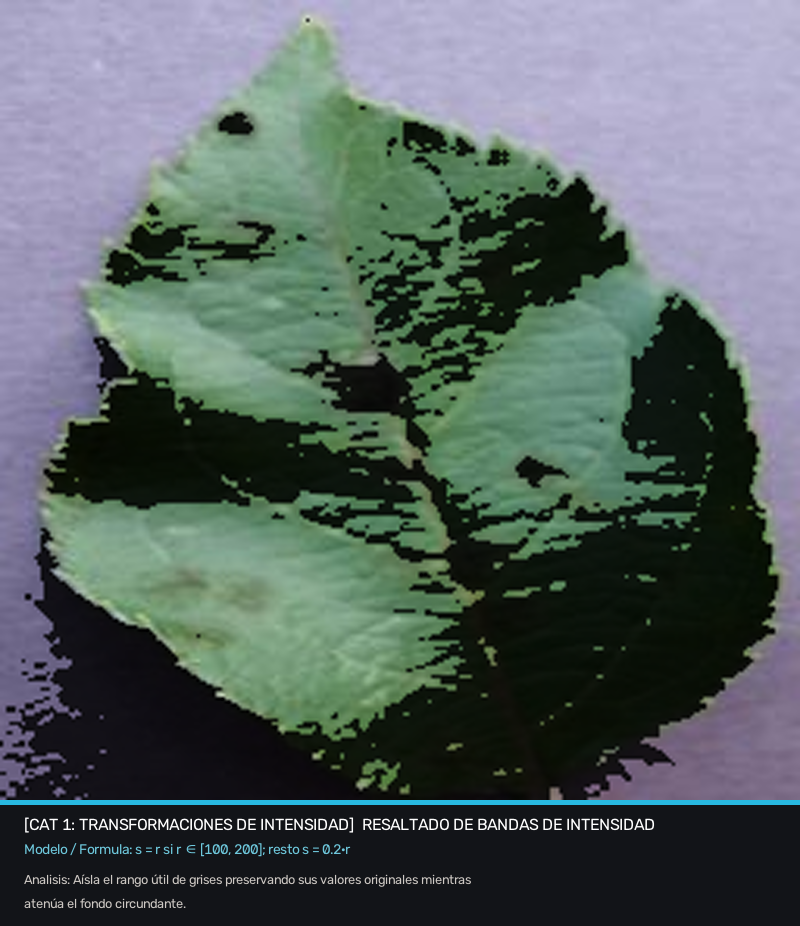
\includegraphics[width=0.78\linewidth]{resultados/individuales/muestra_01/08_banda_intensidad.png}
  \caption{\textbf{Resaltado de Bandas de Intensidad:} Aísla el rango útil de grises preservando sus valores originales mientras atenúa el fondo circundante. \textit{Modelo:} \texttt{s = r si r ∈ [100, 200]; resto s = 0.2·r}.}
  \label{fig:08_banda_intensidad}
\end{figure}

\begin{figure}[htbp]
  \centering
  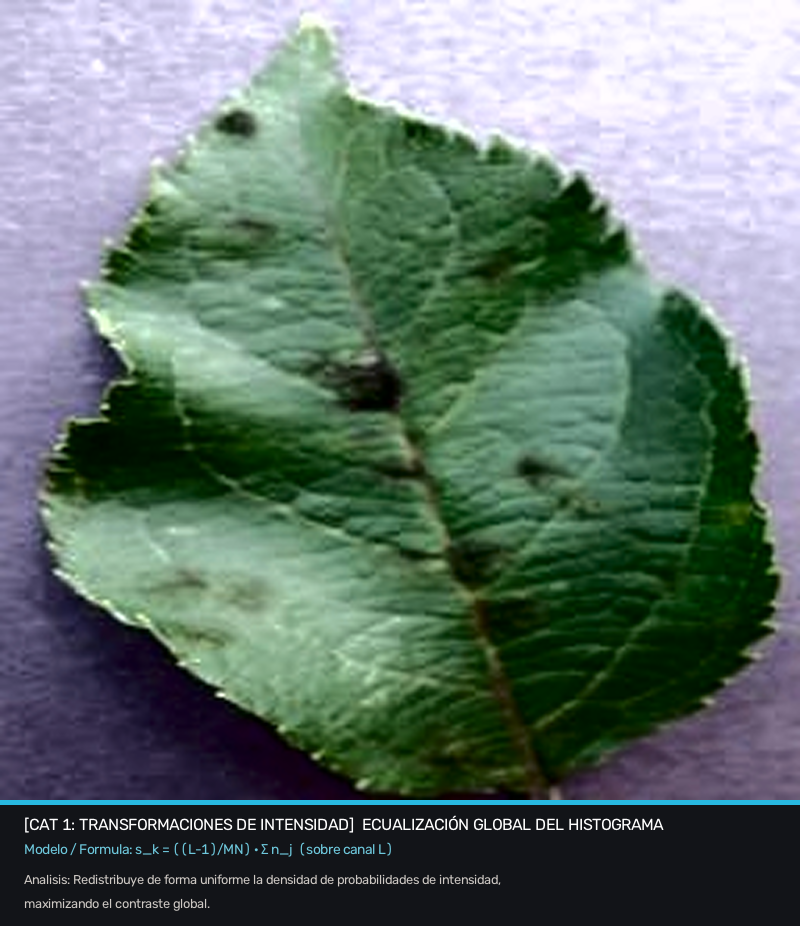
\includegraphics[width=0.78\linewidth]{resultados/individuales/muestra_01/09_ecualizacion_global.png}
  \caption{\textbf{Ecualización Global del Histograma:} Redistribuye de forma uniforme la densidad de probabilidades de intensidad, maximizando el contraste global. \textit{Modelo:} \texttt{s_k = ((L-1)/MN) · Σ n_j  (sobre canal L)}.}
  \label{fig:09_ecualizacion_global}
\end{figure}

\begin{figure}[htbp]
  \centering
  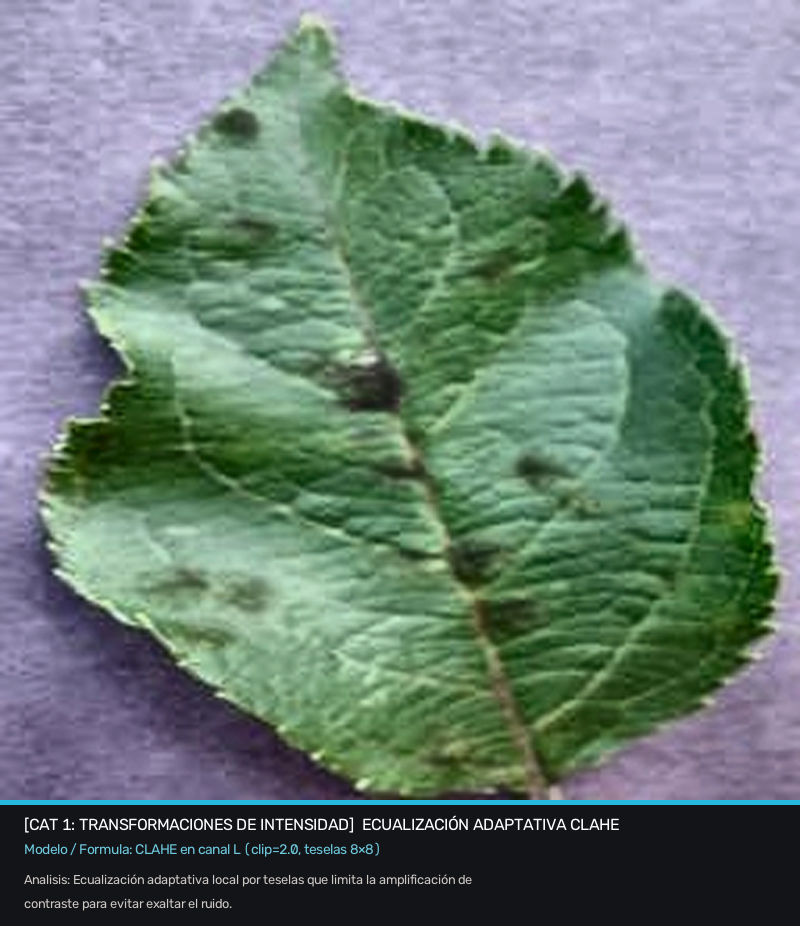
\includegraphics[width=0.78\linewidth]{resultados/individuales/muestra_01/10_ecualizacion_clahe.png}
  \caption{\textbf{Ecualización Adaptativa CLAHE:} Ecualización adaptativa local por teselas que limita la amplificación de contraste para evitar exaltar el ruido. \textit{Modelo:} \texttt{CLAHE en canal L (clip=2.0, teselas 8×8)}.}
  \label{fig:10_ecualizacion_clahe}
\end{figure}


\subsection*{Cat 2: Filtros Estadísticos / De Orden}

\begin{figure}[htbp]
  \centering
  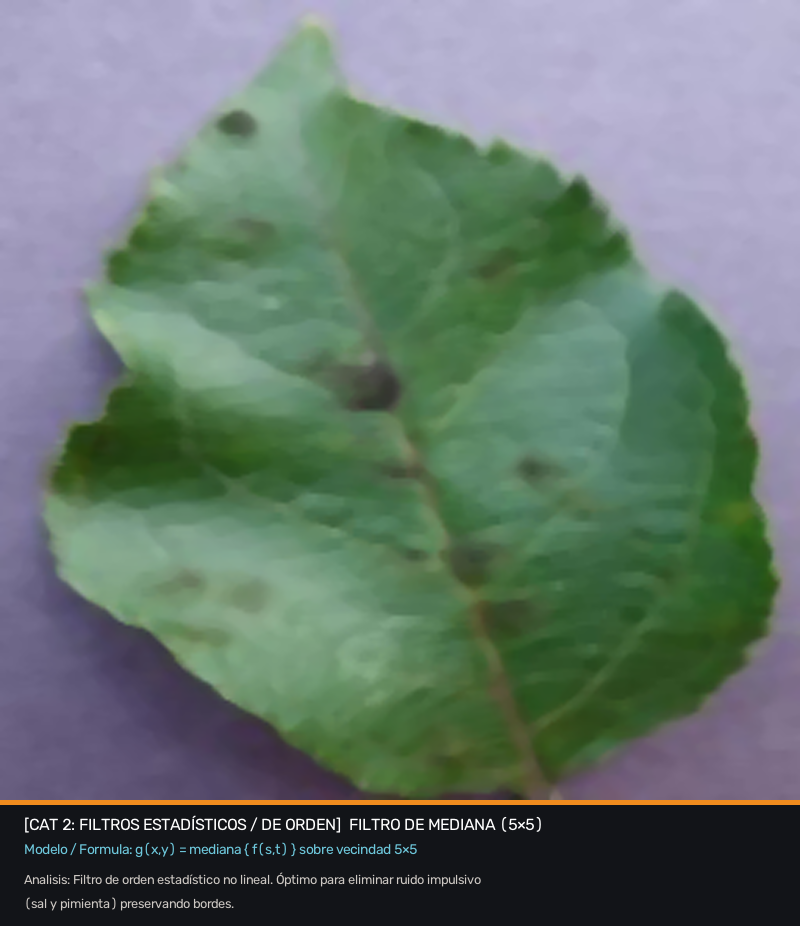
\includegraphics[width=0.78\linewidth]{resultados/individuales/muestra_01/11_filtro_mediana.png}
  \caption{\textbf{Filtro de Mediana (5×5):} Filtro de orden estadístico no lineal. Óptimo para eliminar ruido impulsivo (sal y pimienta) preservando bordes. \textit{Modelo:} \texttt{g(x,y) = mediana { f(s,t) } sobre vecindad 5×5}.}
  \label{fig:11_filtro_mediana}
\end{figure}

\begin{figure}[htbp]
  \centering
  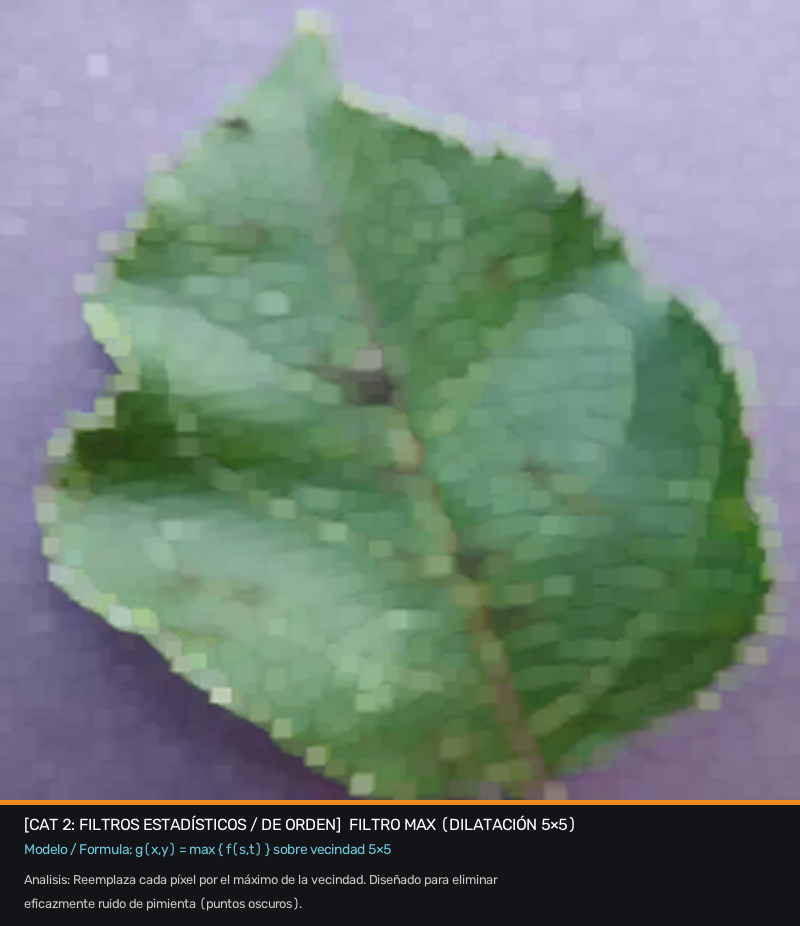
\includegraphics[width=0.78\linewidth]{resultados/individuales/muestra_01/12_filtro_max.png}
  \caption{\textbf{Filtro MAX (Dilatación 5×5):} Reemplaza cada píxel por el máximo de la vecindad. Diseñado para eliminar eficazmente ruido de pimienta (puntos oscuros). \textit{Modelo:} \texttt{g(x,y) = max { f(s,t) } sobre vecindad 5×5}.}
  \label{fig:12_filtro_max}
\end{figure}

\begin{figure}[htbp]
  \centering
  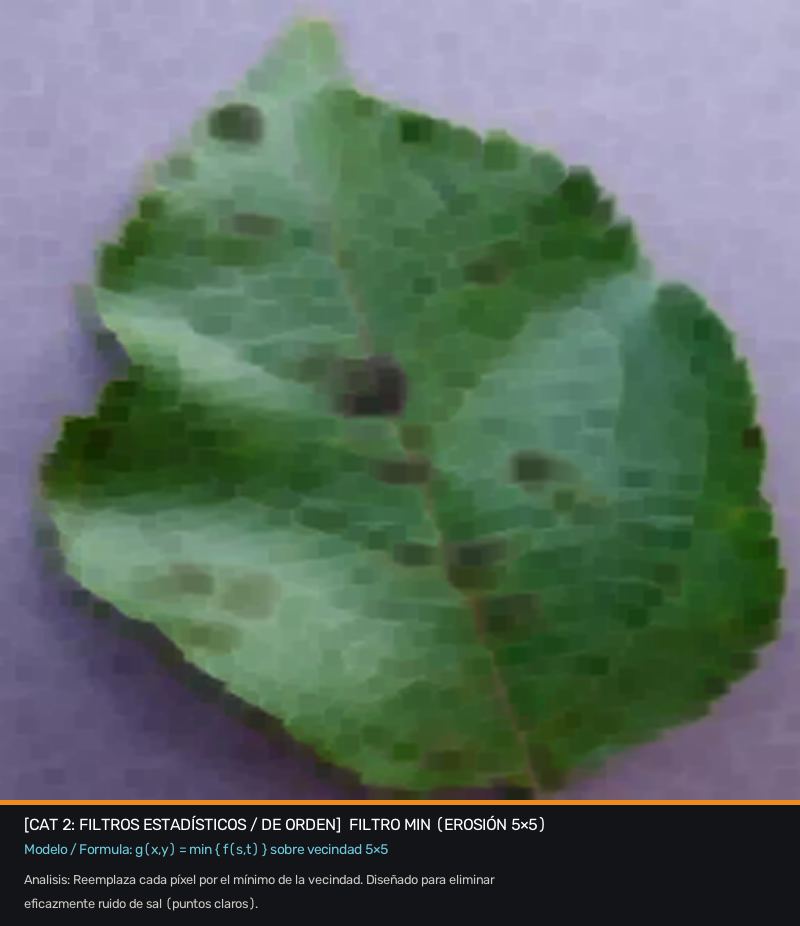
\includegraphics[width=0.78\linewidth]{resultados/individuales/muestra_01/13_filtro_min.png}
  \caption{\textbf{Filtro MIN (Erosión 5×5):} Reemplaza cada píxel por el mínimo de la vecindad. Diseñado para eliminar eficazmente ruido de sal (puntos claros). \textit{Modelo:} \texttt{g(x,y) = min { f(s,t) } sobre vecindad 5×5}.}
  \label{fig:13_filtro_min}
\end{figure}

\begin{figure}[htbp]
  \centering
  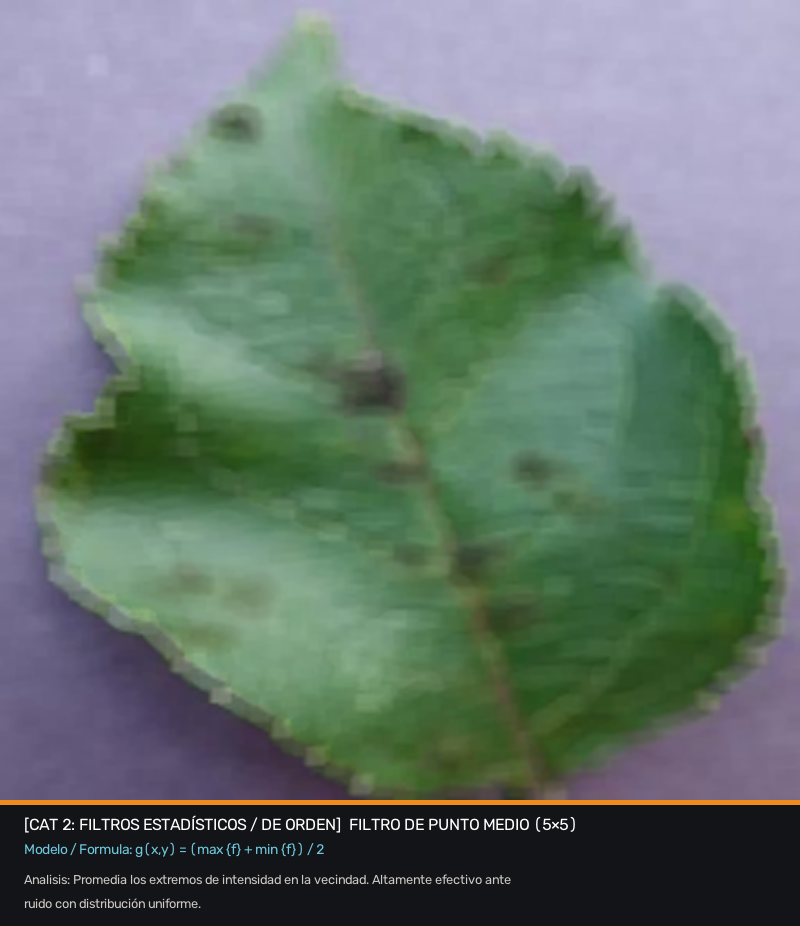
\includegraphics[width=0.78\linewidth]{resultados/individuales/muestra_01/14_filtro_punto_medio.png}
  \caption{\textbf{Filtro de Punto Medio (5×5):} Promedia los extremos de intensidad en la vecindad. Altamente efectivo ante ruido con distribución uniforme. \textit{Modelo:} \texttt{g(x,y) = (max {f} + min {f}) / 2}.}
  \label{fig:14_filtro_punto_medio}
\end{figure}

\begin{figure}[htbp]
  \centering
  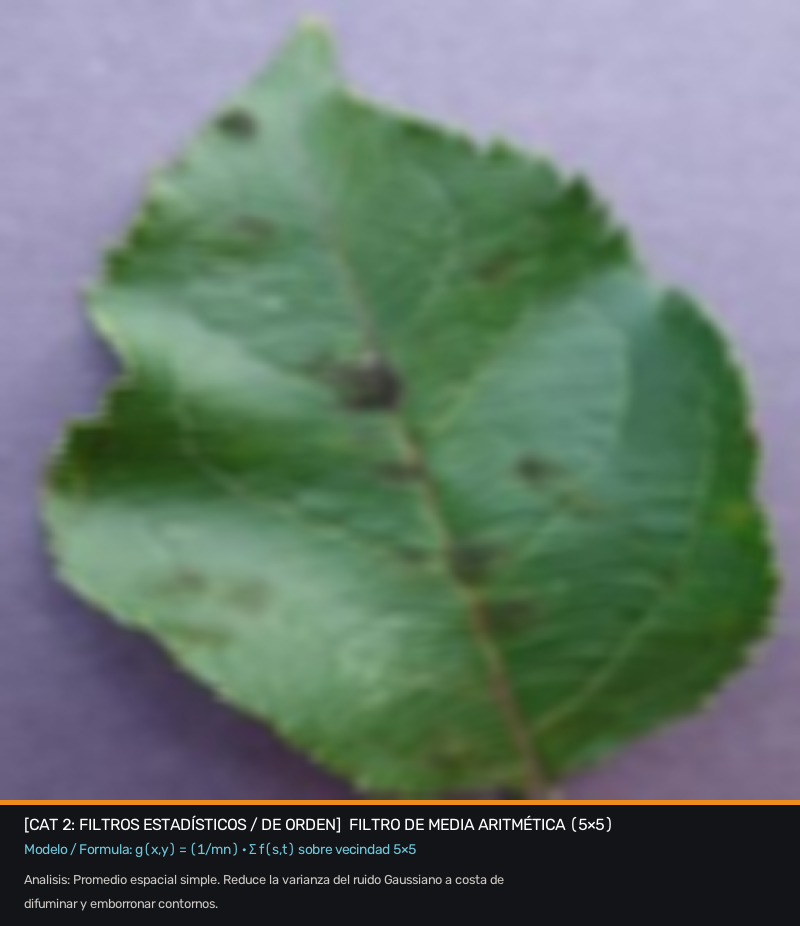
\includegraphics[width=0.78\linewidth]{resultados/individuales/muestra_01/15_media_aritmetica.png}
  \caption{\textbf{Filtro de Media Aritmética (5×5):} Promedio espacial simple. Reduce la varianza del ruido Gaussiano a costa de difuminar y emborronar contornos. \textit{Modelo:} \texttt{g(x,y) = (1/mn) · Σ f(s,t) sobre vecindad 5×5}.}
  \label{fig:15_media_aritmetica}
\end{figure}

\begin{figure}[htbp]
  \centering
  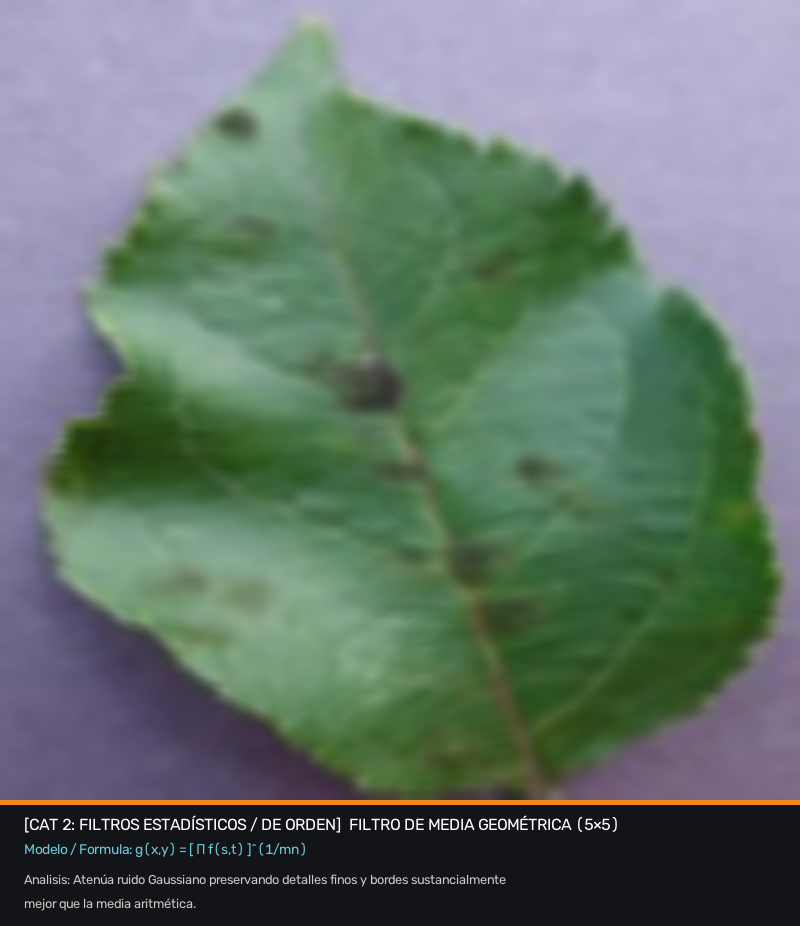
\includegraphics[width=0.78\linewidth]{resultados/individuales/muestra_01/16_media_geometrica.png}
  \caption{\textbf{Filtro de Media Geométrica (5×5):} Atenúa ruido Gaussiano preservando detalles finos y bordes sustancialmente mejor que la media aritmética. \textit{Modelo:} \texttt{g(x,y) = [ Π f(s,t) ]^(1/mn)}.}
  \label{fig:16_media_geometrica}
\end{figure}


\subsection*{Cat 3: Filtros Suavizantes (Pasabajas)}

\begin{figure}[htbp]
  \centering
  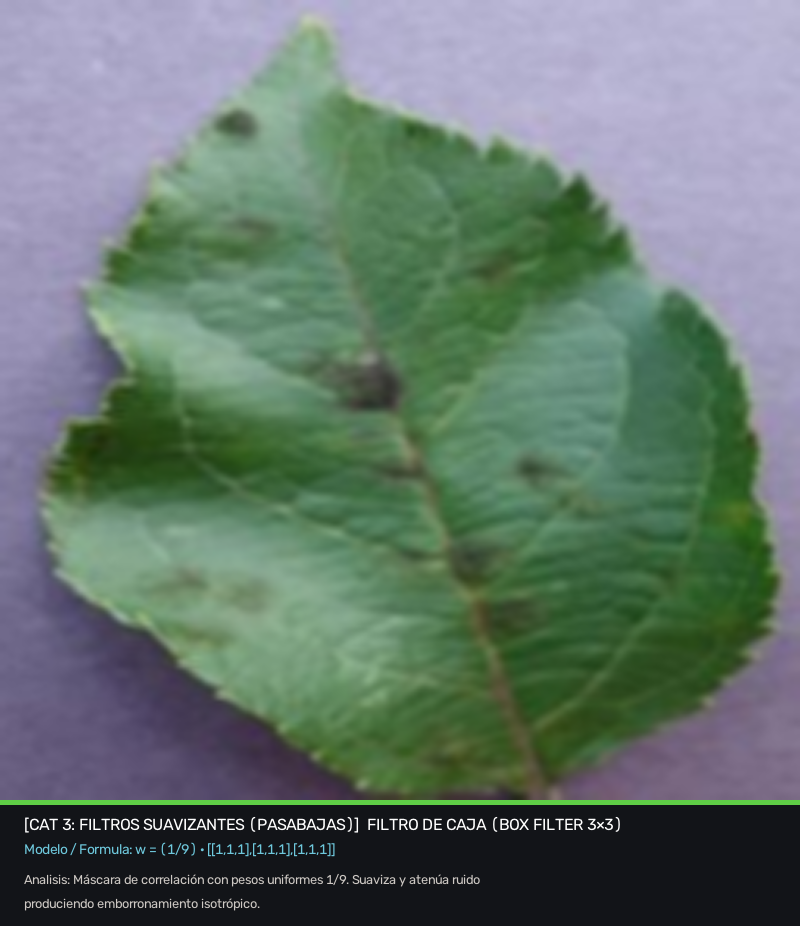
\includegraphics[width=0.78\linewidth]{resultados/individuales/muestra_01/17_filtro_caja.png}
  \caption{\textbf{Filtro de Caja (Box Filter 3×3):} Máscara de correlación con pesos uniformes 1/9. Suaviza y atenúa ruido produciendo emborronamiento isotrópico. \textit{Modelo:} \texttt{w = (1/9) · [[1,1,1],[1,1,1],[1,1,1]]}.}
  \label{fig:17_filtro_caja}
\end{figure}

\begin{figure}[htbp]
  \centering
  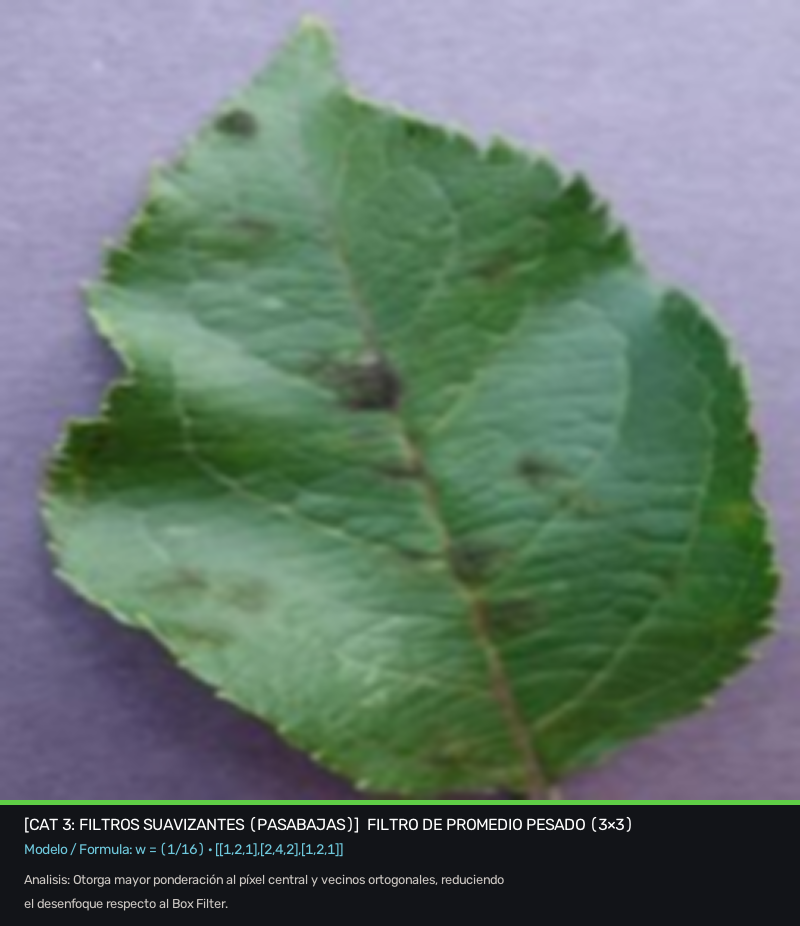
\includegraphics[width=0.78\linewidth]{resultados/individuales/muestra_01/18_promedio_pesado.png}
  \caption{\textbf{Filtro de Promedio Pesado (3×3):} Otorga mayor ponderación al píxel central y vecinos ortogonales, reduciendo el desenfoque respecto al Box Filter. \textit{Modelo:} \texttt{w = (1/16) · [[1,2,1],[2,4,2],[1,2,1]]}.}
  \label{fig:18_promedio_pesado}
\end{figure}

\begin{figure}[htbp]
  \centering
  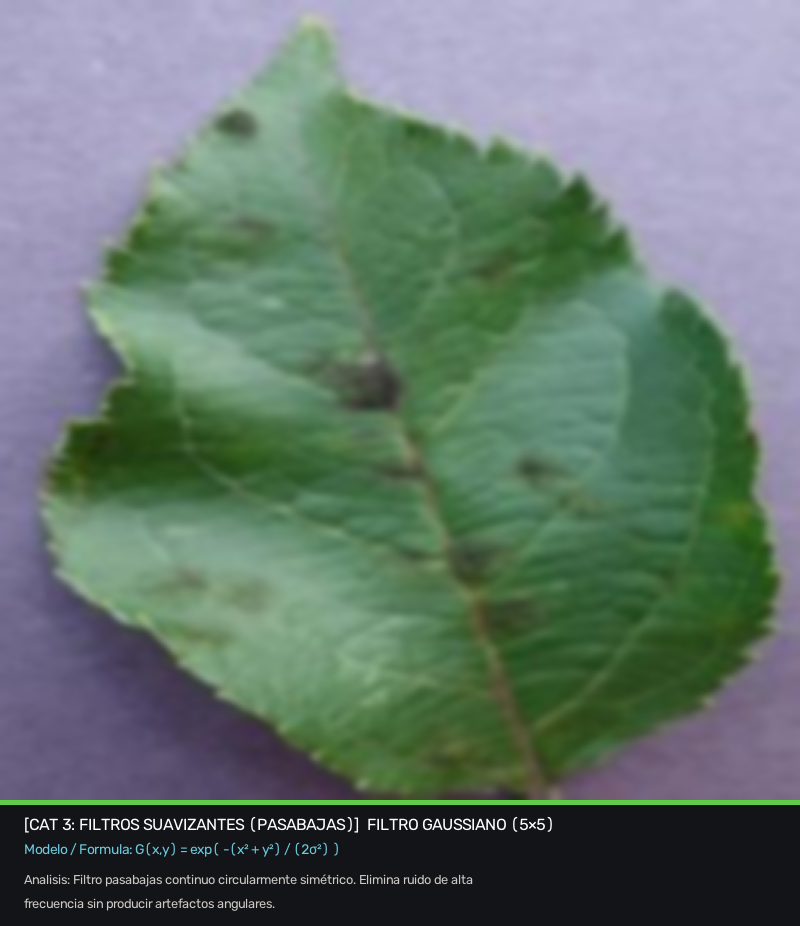
\includegraphics[width=0.78\linewidth]{resultados/individuales/muestra_01/19_filtro_gaussiano.png}
  \caption{\textbf{Filtro Gaussiano (5×5):} Filtro pasabajas continuo circularmente simétrico. Elimina ruido de alta frecuencia sin producir artefactos angulares. \textit{Modelo:} \texttt{G(x,y) = exp( -(x² + y²) / (2σ²) )}.}
  \label{fig:19_filtro_gaussiano}
\end{figure}

\begin{figure}[htbp]
  \centering
  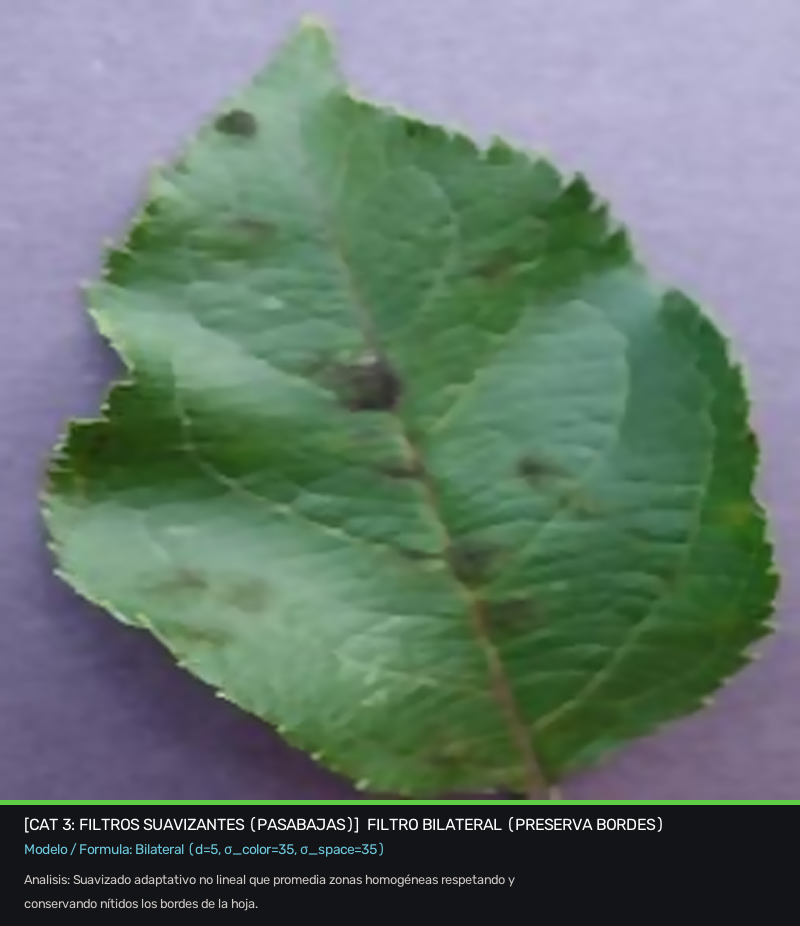
\includegraphics[width=0.78\linewidth]{resultados/individuales/muestra_01/20_filtro_bilateral.png}
  \caption{\textbf{Filtro Bilateral (Preserva Bordes):} Suavizado adaptativo no lineal que promedia zonas homogéneas respetando y conservando nítidos los bordes de la hoja. \textit{Modelo:} \texttt{Bilateral (d=5, σ_color=35, σ_space=35)}.}
  \label{fig:20_filtro_bilateral}
\end{figure}


\subsection*{Cat 4: Filtros Realzantes (Derivadas)}

\begin{figure}[htbp]
  \centering
  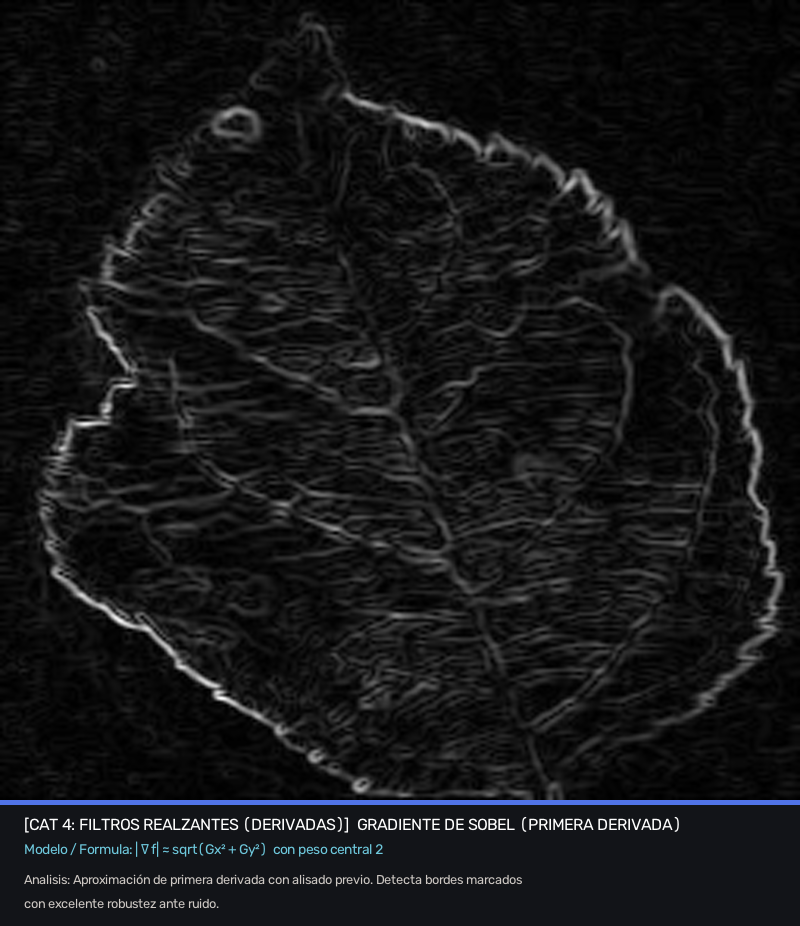
\includegraphics[width=0.78\linewidth]{resultados/individuales/muestra_01/21_sobel_gradiente.png}
  \caption{\textbf{Gradiente de Sobel (Primera Derivada):} Aproximación de primera derivada con alisado previo. Detecta bordes marcados con excelente robustez ante ruido. \textit{Modelo:} \texttt{|∇f| ≈ sqrt(Gx² + Gy²)  con peso central 2}.}
  \label{fig:21_sobel_gradiente}
\end{figure}

\begin{figure}[htbp]
  \centering
  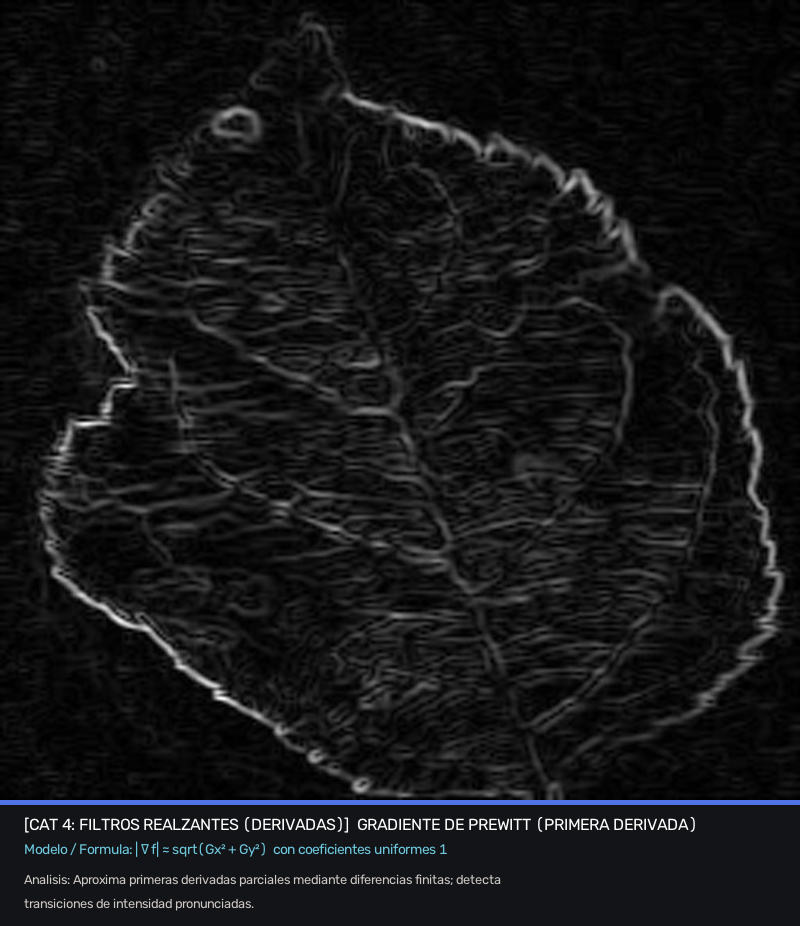
\includegraphics[width=0.78\linewidth]{resultados/individuales/muestra_01/22_prewitt_gradiente.png}
  \caption{\textbf{Gradiente de Prewitt (Primera Derivada):} Aproxima primeras derivadas parciales mediante diferencias finitas; detecta transiciones de intensidad pronunciadas. \textit{Modelo:} \texttt{|∇f| ≈ sqrt(Gx² + Gy²)  con coeficientes uniformes 1}.}
  \label{fig:22_prewitt_gradiente}
\end{figure}

\begin{figure}[htbp]
  \centering
  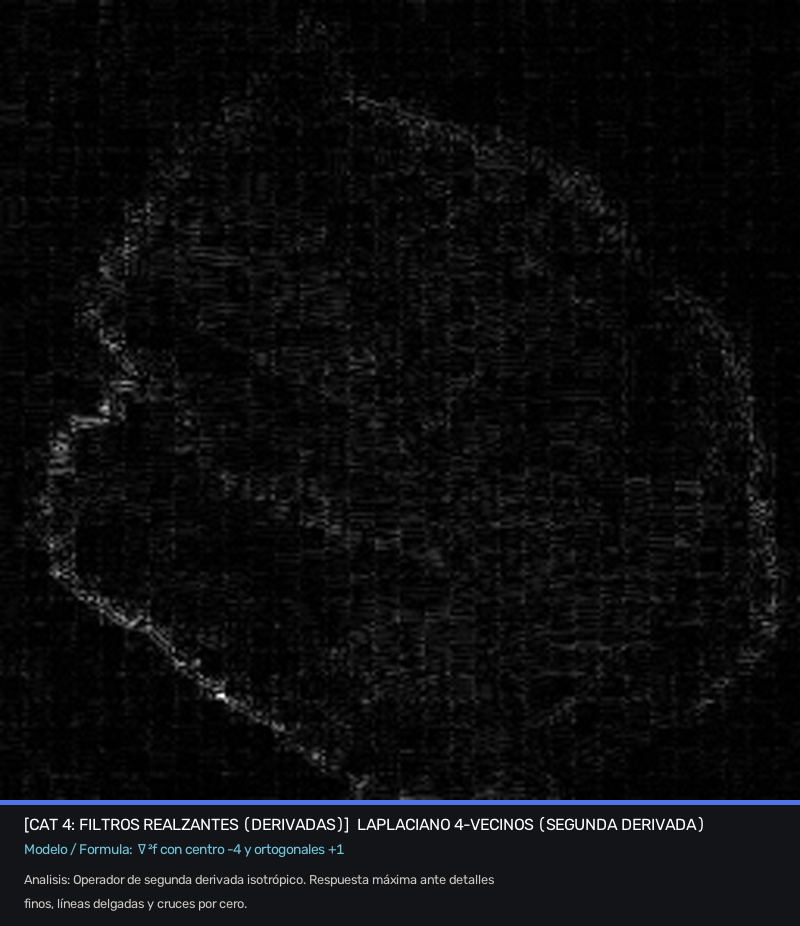
\includegraphics[width=0.78\linewidth]{resultados/individuales/muestra_01/23_laplaciano_4vec.png}
  \caption{\textbf{Laplaciano 4-vecinos (Segunda Derivada):} Operador de segunda derivada isotrópico. Respuesta máxima ante detalles finos, líneas delgadas y cruces por cero. \textit{Modelo:} \texttt{∇²f con centro -4 y ortogonales +1}.}
  \label{fig:23_laplaciano_4vec}
\end{figure}

\begin{figure}[htbp]
  \centering
  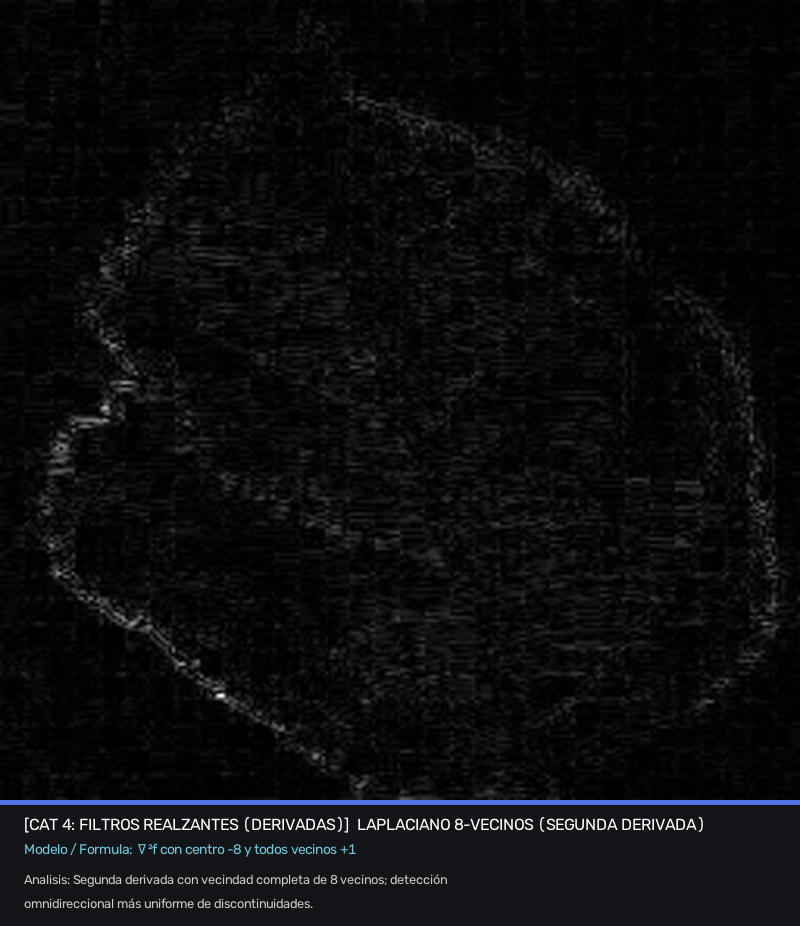
\includegraphics[width=0.78\linewidth]{resultados/individuales/muestra_01/24_laplaciano_8vec.png}
  \caption{\textbf{Laplaciano 8-vecinos (Segunda Derivada):} Segunda derivada con vecindad completa de 8 vecinos; detección omnidireccional más uniforme de discontinuidades. \textit{Modelo:} \texttt{∇²f con centro -8 y todos vecinos +1}.}
  \label{fig:24_laplaciano_8vec}
\end{figure}

\begin{figure}[htbp]
  \centering
  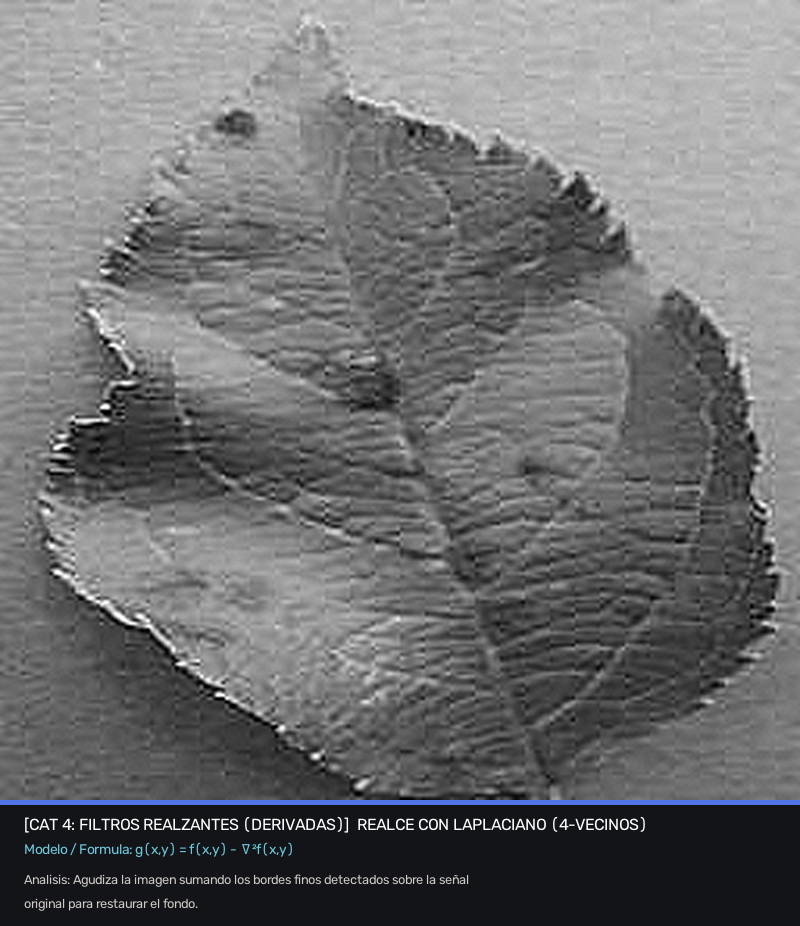
\includegraphics[width=0.78\linewidth]{resultados/individuales/muestra_01/25_realce_laplaciano_4vec.png}
  \caption{\textbf{Realce con Laplaciano (4-vecinos):} Agudiza la imagen sumando los bordes finos detectados sobre la señal original para restaurar el fondo. \textit{Modelo:} \texttt{g(x,y) = f(x,y) - ∇²f(x,y)}.}
  \label{fig:25_realce_laplaciano_4vec}
\end{figure}

\begin{figure}[htbp]
  \centering
  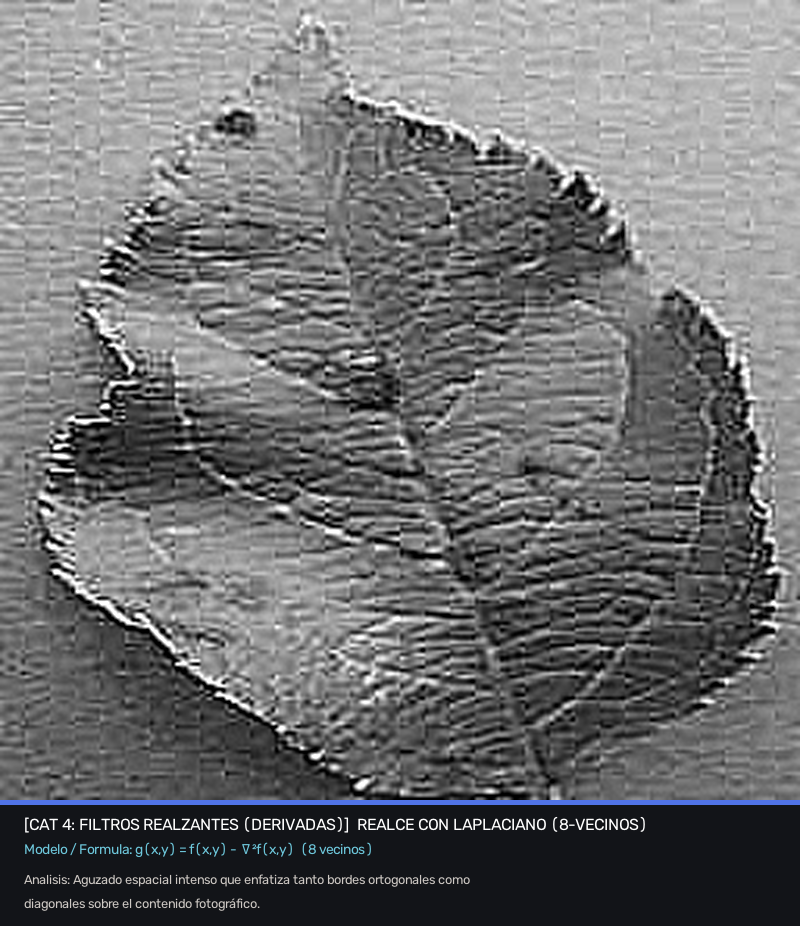
\includegraphics[width=0.78\linewidth]{resultados/individuales/muestra_01/26_realce_laplaciano_8vec.png}
  \caption{\textbf{Realce con Laplaciano (8-vecinos):} Aguzado espacial intenso que enfatiza tanto bordes ortogonales como diagonales sobre el contenido fotográfico. \textit{Modelo:} \texttt{g(x,y) = f(x,y) - ∇²f(x,y)  (8 vecinos)}.}
  \label{fig:26_realce_laplaciano_8vec}
\end{figure}

\begin{figure}[htbp]
  \centering
  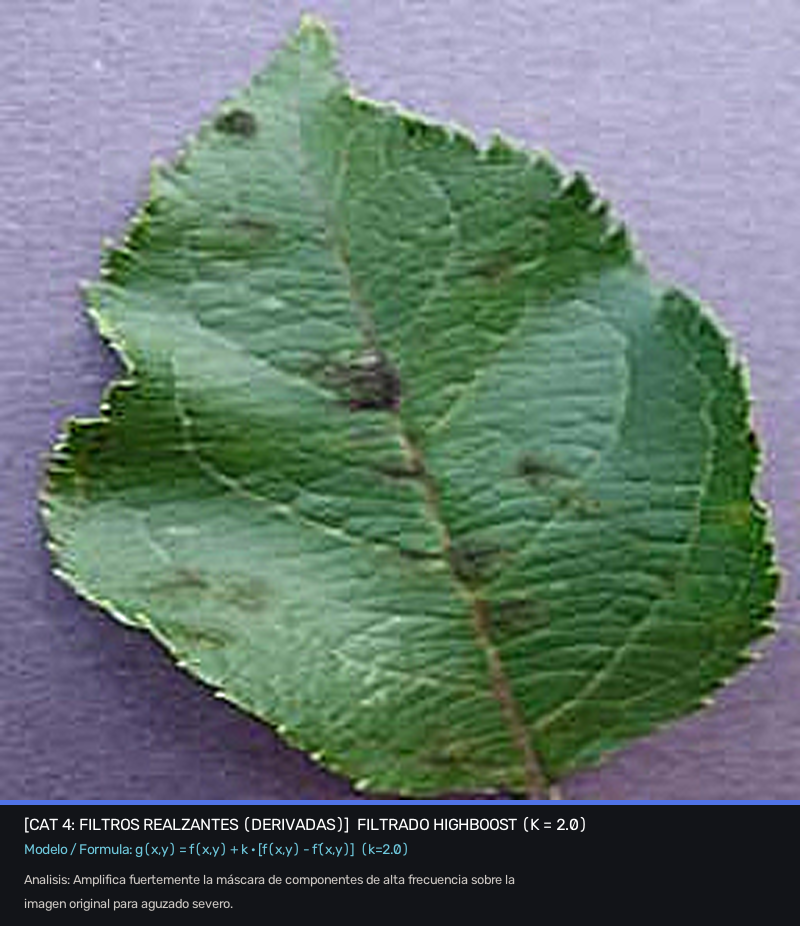
\includegraphics[width=0.78\linewidth]{resultados/individuales/muestra_01/27_highboost.png}
  \caption{\textbf{Filtrado Highboost (k = 2.0):} Amplifica fuertemente la máscara de componentes de alta frecuencia sobre la imagen original para aguzado severo. \textit{Modelo:} \texttt{g(x,y) = f(x,y) + k · [f(x,y) - f̄(x,y)]  (k=2.0)}.}
  \label{fig:27_highboost}
\end{figure}

\begin{figure}[htbp]
  \centering
  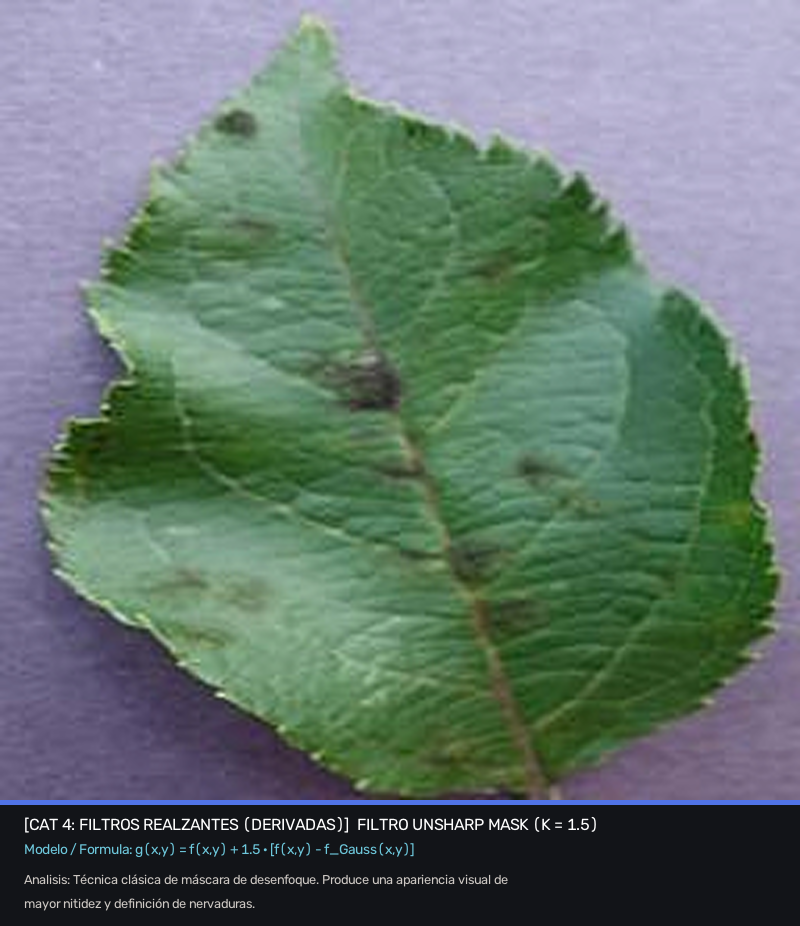
\includegraphics[width=0.78\linewidth]{resultados/individuales/muestra_01/28_unsharp_mask.png}
  \caption{\textbf{Filtro Unsharp Mask (k = 1.5):} Técnica clásica de máscara de desenfoque. Produce una apariencia visual de mayor nitidez y definición de nervaduras. \textit{Modelo:} \texttt{g(x,y) = f(x,y) + 1.5 · [f(x,y) - f_Gauss(x,y)]}.}
  \label{fig:28_unsharp_mask}
\end{figure}

\begin{figure}[htbp]
  \centering
  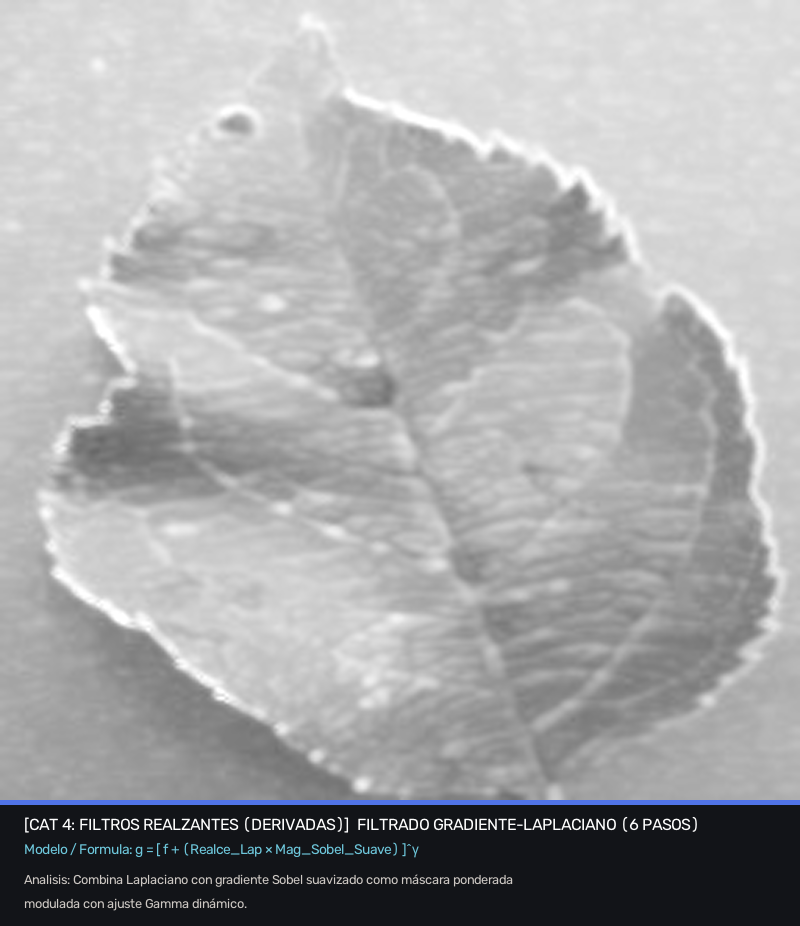
\includegraphics[width=0.78\linewidth]{resultados/individuales/muestra_01/29_gradiente_laplaciano_6pasos.png}
  \caption{\textbf{Filtrado Gradiente-Laplaciano (6 Pasos):} Combina Laplaciano con gradiente Sobel suavizado como máscara ponderada modulada con ajuste Gamma dinámico. \textit{Modelo:} \texttt{g = [ f + (Realce_Lap × Mag_Sobel_Suave) ]^γ}.}
  \label{fig:29_gradiente_laplaciano_6pasos}
\end{figure}


\subsection*{Cat 5: Segmentación y Bordes Avanzados}

\begin{figure}[htbp]
  \centering
  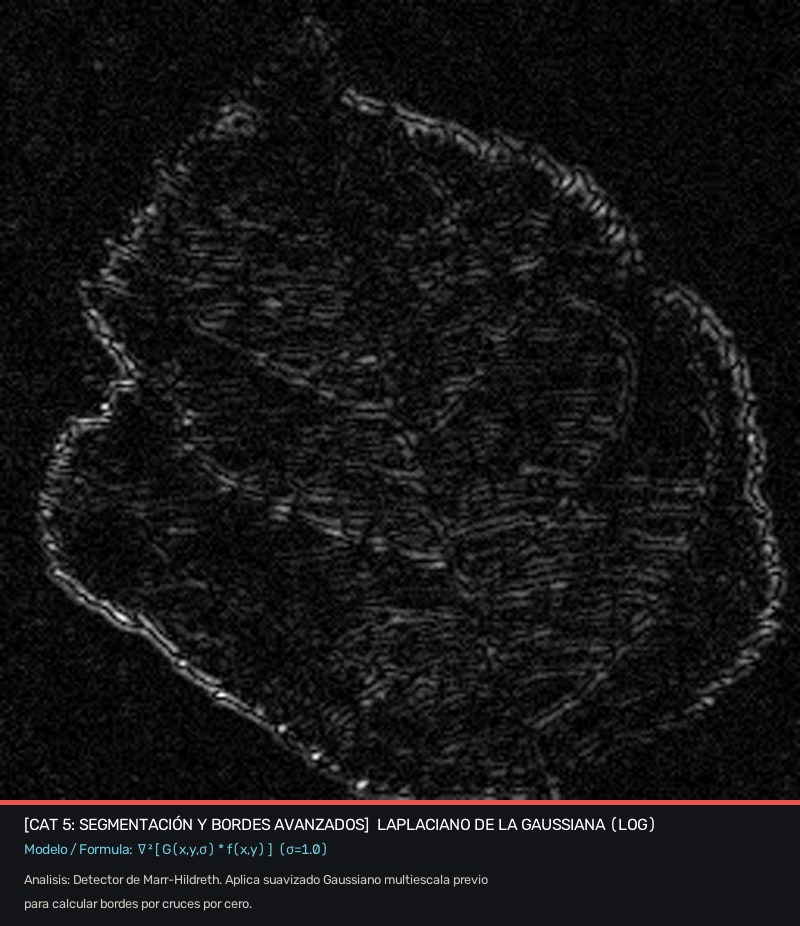
\includegraphics[width=0.78\linewidth]{resultados/individuales/muestra_01/30_log_marr_hildreth.png}
  \caption{\textbf{Laplaciano de la Gaussiana (LoG):} Detector de Marr-Hildreth. Aplica suavizado Gaussiano multiescala previo para calcular bordes por cruces por cero. \textit{Modelo:} \texttt{∇² [ G(x,y,σ) * f(x,y) ]  (σ=1.0)}.}
  \label{fig:30_log_marr_hildreth}
\end{figure}

\begin{figure}[htbp]
  \centering
  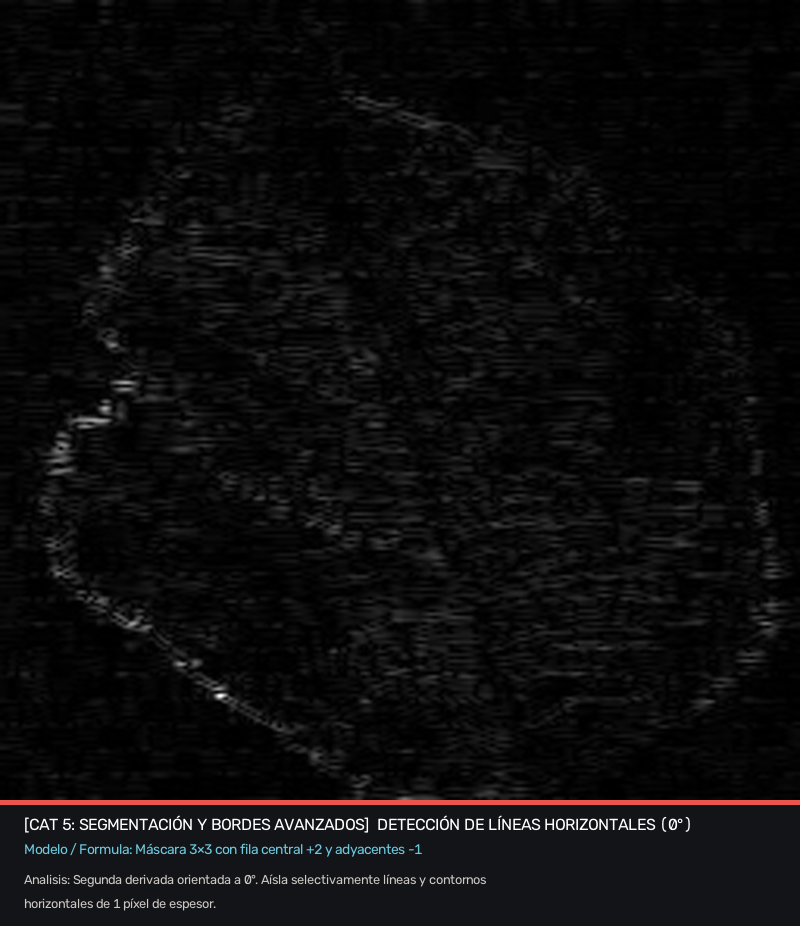
\includegraphics[width=0.78\linewidth]{resultados/individuales/muestra_01/31_lineas_0_horizontal.png}
  \caption{\textbf{Detección de Líneas Horizontales (0°):} Segunda derivada orientada a 0°. Aísla selectivamente líneas y contornos horizontales de 1 píxel de espesor. \textit{Modelo:} \texttt{Máscara 3×3 con fila central +2 y adyacentes -1}.}
  \label{fig:31_lineas_0_horizontal}
\end{figure}

\begin{figure}[htbp]
  \centering
  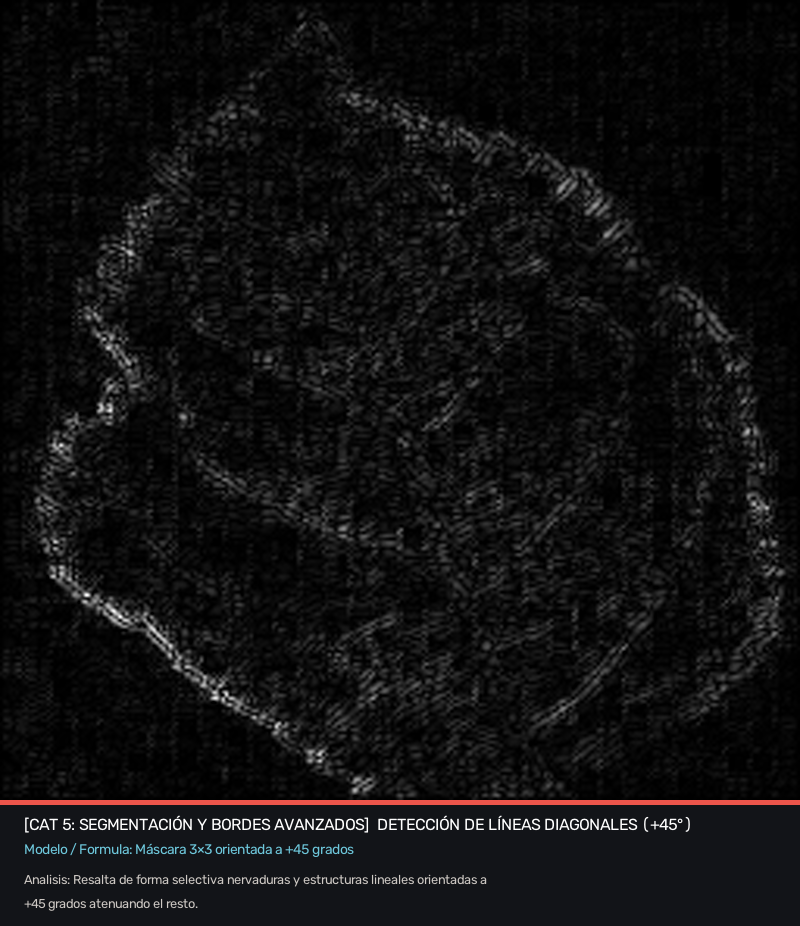
\includegraphics[width=0.78\linewidth]{resultados/individuales/muestra_01/32_lineas_45_diagonal.png}
  \caption{\textbf{Detección de Líneas Diagonales (+45°):} Resalta de forma selectiva nervaduras y estructuras lineales orientadas a +45 grados atenuando el resto. \textit{Modelo:} \texttt{Máscara 3×3 orientada a +45 grados}.}
  \label{fig:32_lineas_45_diagonal}
\end{figure}

\begin{figure}[htbp]
  \centering
  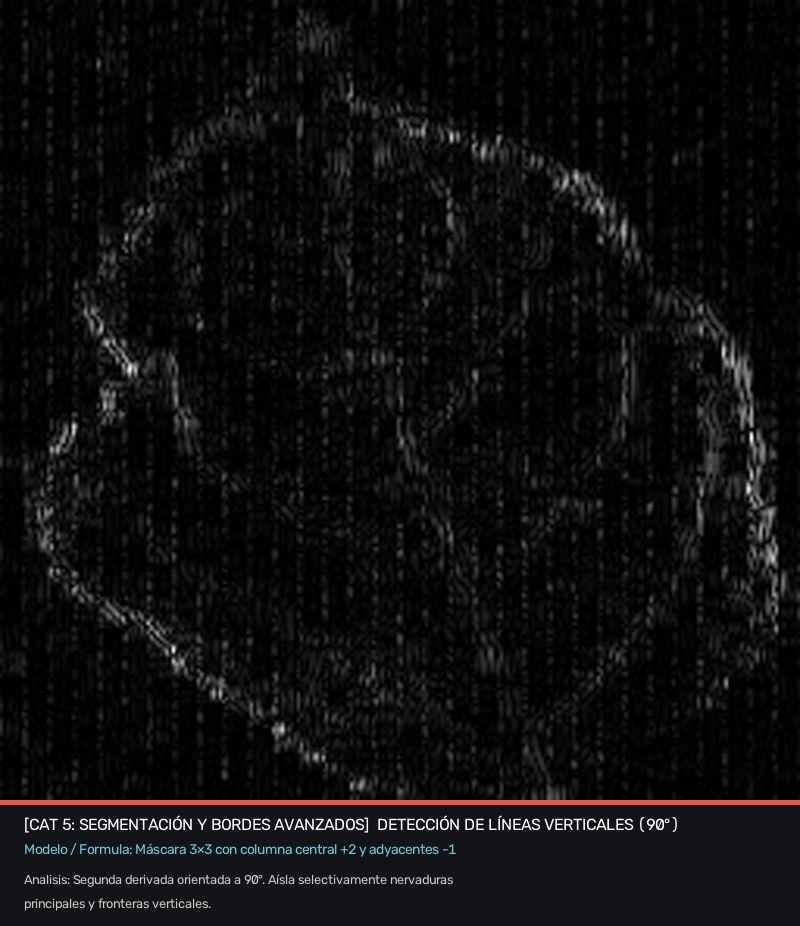
\includegraphics[width=0.78\linewidth]{resultados/individuales/muestra_01/33_lineas_90_vertical.png}
  \caption{\textbf{Detección de Líneas Verticales (90°):} Segunda derivada orientada a 90°. Aísla selectivamente nervaduras principales y fronteras verticales. \textit{Modelo:} \texttt{Máscara 3×3 con columna central +2 y adyacentes -1}.}
  \label{fig:33_lineas_90_vertical}
\end{figure}

\begin{figure}[htbp]
  \centering
  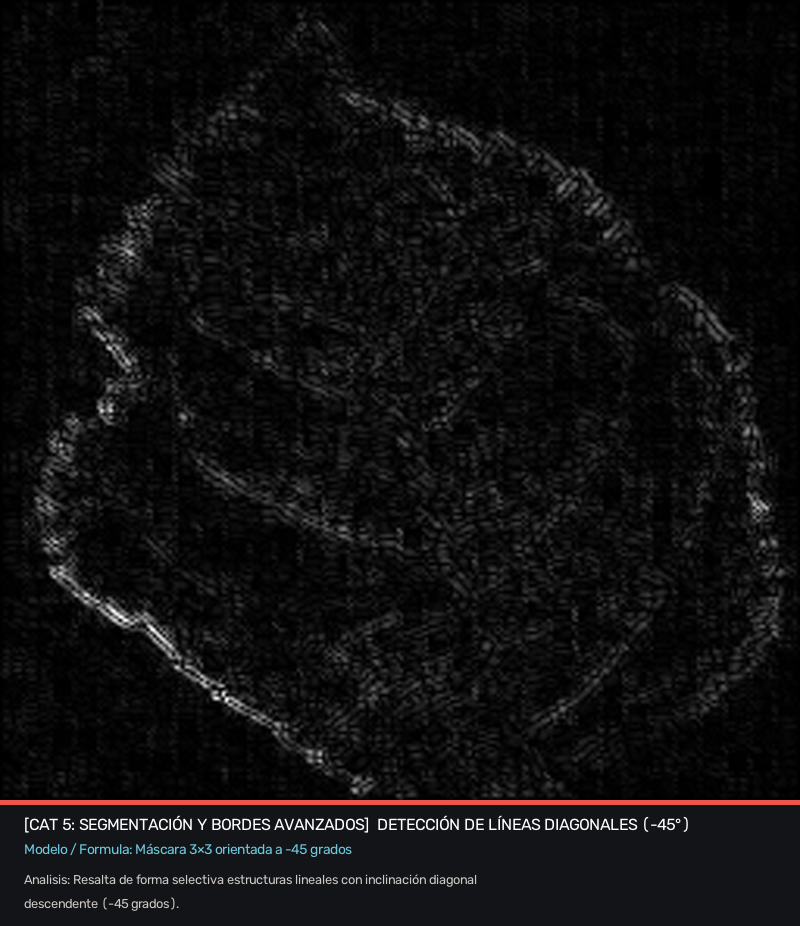
\includegraphics[width=0.78\linewidth]{resultados/individuales/muestra_01/34_lineas_menos45_diagonal.png}
  \caption{\textbf{Detección de Líneas Diagonales (-45°):} Resalta de forma selectiva estructuras lineales con inclinación diagonal descendente (-45 grados). \textit{Modelo:} \texttt{Máscara 3×3 orientada a -45 grados}.}
  \label{fig:34_lineas_menos45_diagonal}
\end{figure}

\begin{figure}[htbp]
  \centering
  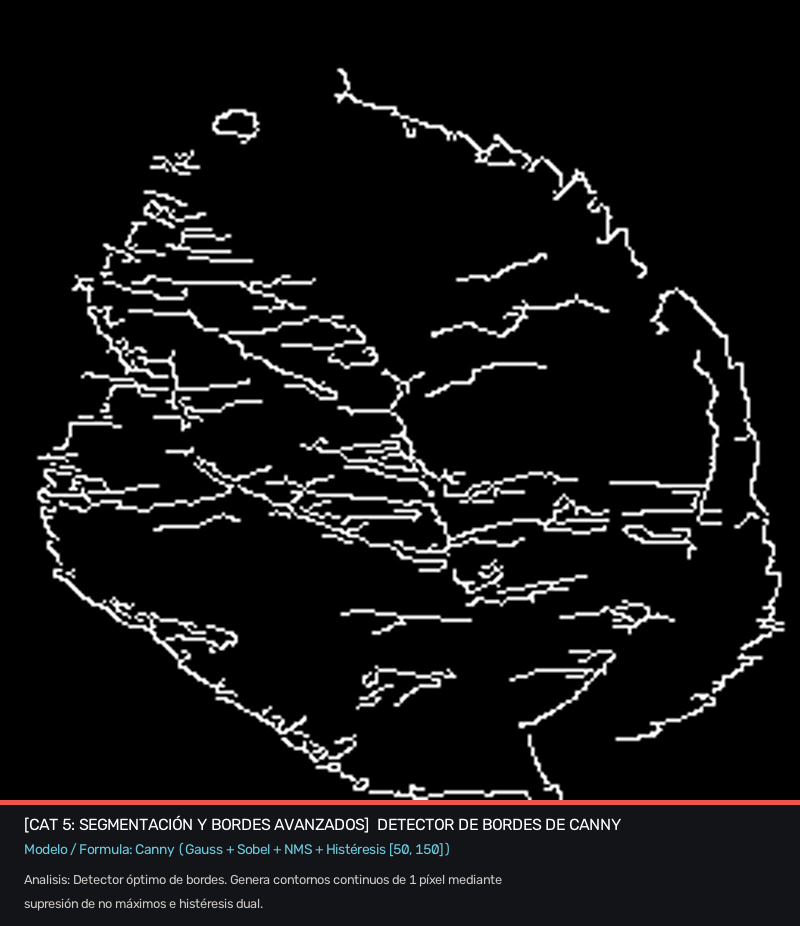
\includegraphics[width=0.78\linewidth]{resultados/individuales/muestra_01/35_detector_canny.png}
  \caption{\textbf{Detector de Bordes de Canny:} Detector óptimo de bordes. Genera contornos continuos de 1 píxel mediante supresión de no máximos e histéresis dual. \textit{Modelo:} \texttt{Canny (Gauss + Sobel + NMS + Histéresis [50, 150])}.}
  \label{fig:35_detector_canny}
\end{figure}


\subsection*{Pipeline de Preprocesamiento Integrado}

\begin{figure}[htbp]
  \centering
  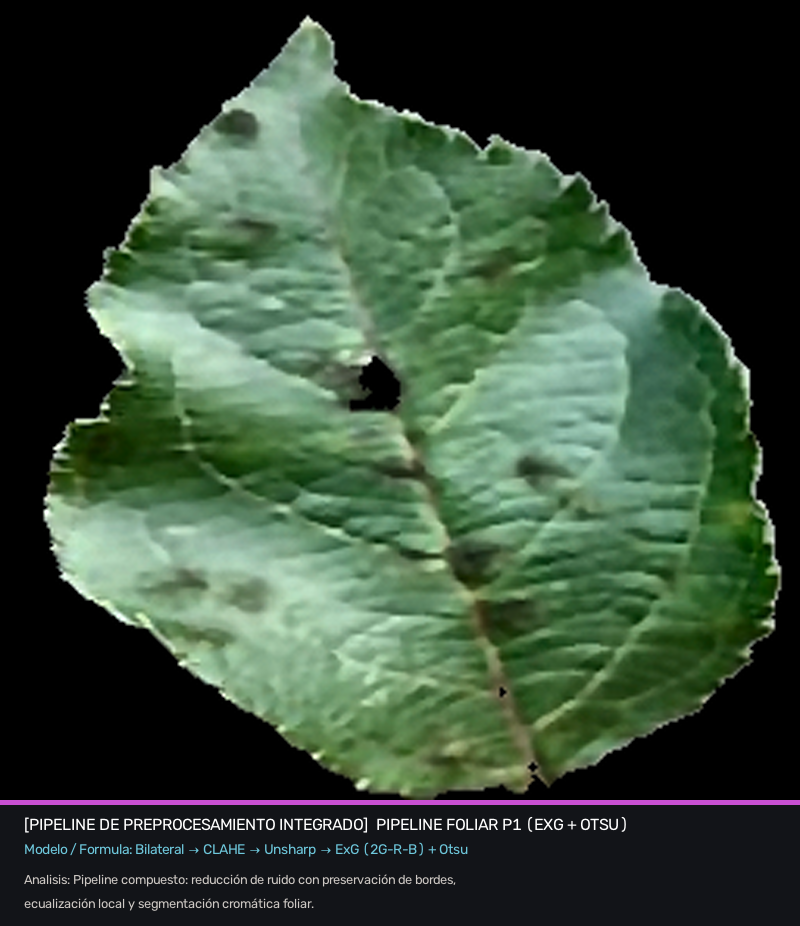
\includegraphics[width=0.78\linewidth]{resultados/individuales/muestra_01/36_pipeline_foliar_exg.png}
  \caption{\textbf{Pipeline Foliar P1 (ExG + Otsu):} Pipeline compuesto: reducción de ruido con preservación de bordes, ecualización local y segmentación cromática foliar. \textit{Modelo:} \texttt{Bilateral → CLAHE → Unsharp → ExG (2G-R-B) + Otsu}.}
  \label{fig:36_pipeline_foliar_exg}
\end{figure}
